% UTF-8 encoding
% Compile with latex+dvipdfmx, pdflatex, xelatex or lualatex

\documentclass[UTF8]{ctexart}
\usepackage{graphicx}
\usepackage{amssymb}
\usepackage{amsmath}
\usepackage{subfigure}
\usepackage{geometry}
\usepackage{caption}

\newcommand{\true}{{\rm T}}
\newcommand{\false}{{\rm F}}
\newcommand{\snatural}{\mathbb{N}}
\newcommand{\sinteger}{\mathbb{Z}}
\newcommand{\srational}{\mathbb{Q}}
\newcommand{\sreal}{\mathbb{R}}

\title{离散数学——第九周作业}
\author{计83  刘轩奇  2018011025}
\date{2019.11.08}

\geometry{left=2.0cm, right=2.0cm, top=2.5cm, bottom=2.5cm}

\begin{document}

\maketitle

\paragraph{9.1}\label{9.1}
列出下列集合所有的元素

(4) $A_4 = \{ z|z= \{ x,y \} \land x \in \sinteger \land y \in \sinteger \land 0 \le x \le 2 \land -2 \le 2 \le 1 \} $

\paragraph{解}
(4) $A_4 = \{ \{ -2,0 \} , \{ -2,1 \} , \{ -2,2 \} , \{ -1,0 \} , \{ -1,1 \} , \{ -1,2 \} , \{ 0 \} , \{ 0,1 \} , \{ 0,2 \} , \{ 1 \} , \{ 1,2 \} \} $

\paragraph{9.2}\label{9.2}
写出下列集合的表达式

(4) $\{3,5,7,11,13,17,19,23,29,\cdots\}$

\paragraph{解}
(4) $A_4 = \{ x|x \in \snatural \land x>2 \land ( \forall y)(y \in \snatural \land y>1 \rightarrow ( \forall z)(z \in \snatural \land z>1 \rightarrow yz \neq x)) \} $

\paragraph{9.3}\label{9.3}
给出集合$A,B,C$的例子,使$A \in B$, $B \in C$但$A \notin C$。

\paragraph{答}
$A = \varnothing, B = \{ \varnothing \} , C = \{ \{ \varnothing \} \} $

\paragraph{9.4}\label{9.4}
给出集合$A,B,C$的例子,使$A \in B$, $B \in C$且$A \in C$。

\paragraph{答}
$A = \varnothing, B = \{ \varnothing \} , C = \{ \varnothing, \{ \varnothing \} \} $

\paragraph{9.6}\label{9.6}
对任意的集合$A,B$和$C$,下列命题是否为真,若真则证明之。若假则举反例。

(2) 若$A \in B$且$B \subseteq C$,则$A \subseteq C$

(4) 若$A \in B$且$B \nsubseteq C$,则$A \notin C$

\paragraph{解}
(2) 假。反例:$A = \{ \varnothing \} , B = C = \{ \{ \varnothing \} \} $

(4) 假。反例:$A = \varnothing, B = \{ \varnothing \} , C= \{ \varnothing, \{ \{ \varnothing \} \} \} $

\paragraph{9.7}\label{9.7}
写出下列集合的幂集和笛卡尔积

(1) $\{ a, \{ a \} \} $的幂集

(3) $ \{ \varnothing, a, \{ b \} \} $的幂集

(5) $ P(P(\varnothing)) \times P(P(\varnothing)) $

\paragraph{解}
(1) $P( \{ a, \{ a \} \} ) = \{ \varnothing, \{ a \} , \{ \{ a \} \} , \{ a, \{ a \} \} \} $

(3) $P( \{ \varnothing, a, \{ b \} \} ) = \{ \varnothing, \{ \varnothing \} , \{ a \} , \{ \{ b \} \} , \{ \varnothing, a \} , \{ \varnothing, \{ b \} \} , \{ a, \{ b \} \} , \{ \varnothing, a, \{ b \} \} \} $

(5) 
\begin{align*}
    & P(P(\varnothing)) \times P(P(\varnothing)) \\
    & = P( \{ \varnothing \} ) \times P( \{ \varnothing \} ) \\
    & = \{ \varnothing, \{ \varnothing \} \} \times \{ \varnothing, \{ \varnothing \} \} \\
    & =  \{ \langle \varnothing, \varnothing \rangle , \langle \varnothing, \{ \varnothing \} \rangle , \langle \{ \varnothing \} , \varnothing \rangle , \langle \{ \varnothing \} , \{ \varnothing \} \rangle \} 
\end{align*}

\paragraph{9.8}\label{9.8}
设$B = P(P(P(\varnothing)))$

(1) 是否$\varnothing \in B$?是否$\varnothing \subseteq B$?

(3) 是否$\{\{\varnothing \}\}\in B$?是否$\{\{\varnothing \}\} \subseteq B$?

\paragraph{解}
$$ B = P(P(P(\varnothing))) = P(P( \{ \varnothing \} )) = P( \{ \varnothing, \{ \varnothing \} \} ) = \{ \varnothing, \{ \varnothing \} , \{ \{ \varnothing \} \} , \{ \varnothing, \{ \varnothing \} \} \} $$

(1) $ \varnothing \in B, \varnothing\subseteq B $

(3) $ \{ \{ \varnothing \} \} \in B, \{ \{ \varnothing \} \} \subseteq B $
\paragraph{9.9}\label{9.9}
画出下列集合的文氏图:

(1) $(-A) \cap (-B)$

(3) $A \oplus (B \cup C)$

\paragraph{解} 如图 9.9 所示。

\begin{figure}[!htb]
    \centering
    \begin{minipage}[t]{0.305\textwidth}
    \centering
    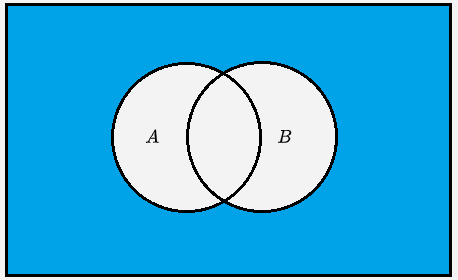
\includegraphics[width=1\textwidth]{9-9-1.png}
    \caption*{(1)}
    \end{minipage}
    \begin{minipage}[t]{0.305\textwidth}
    \centering
    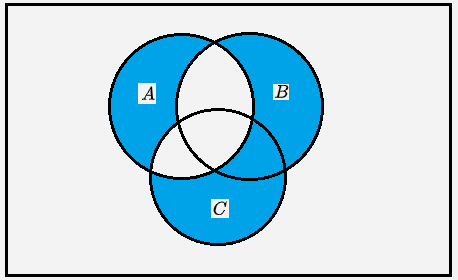
\includegraphics[width=1\textwidth]{9-9-3.png}
    \caption*{(3)}
    \end{minipage}
    \caption*{图 9.9}
\end{figure}    

\paragraph{9.10}\label{9.10}
用公式表示下列文氏图(题图9.10 (1))中的集合:

\begin{figure}[!htb]
    \centering
    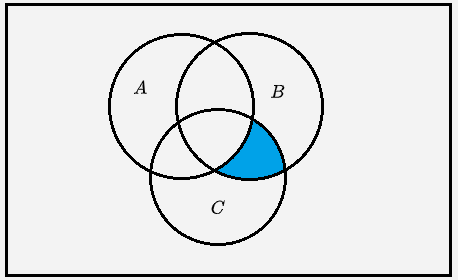
\includegraphics[width=0.305\textwidth]{9-10-1.png}
    \caption*{题图 9.10 (1)}
\end{figure}    

\paragraph{答} (1) $(B \cap C)-A$

\paragraph{9.11}\label{9.11}
化简下列各式:

(2) $ \{ \varnothing, \{ \varnothing \} \} - \varnothing $

(4) $ \{ \varnothing, \{ \varnothing \} \} - \{ \{ \varnothing \} \} $

\paragraph{解}
(2) $ \{ \varnothing, \{ \varnothing \} \} - \varnothing = \{ \varnothing, \{ \varnothing \} \} $

(4) $ \{ \varnothing, \{ \varnothing \} \} - \{ \{ \varnothing \} \} = \{ \varnothing \} $

\paragraph{9.12}\label{9.12}
设全集 $E=\{1,2,3,4,5\}$,集合$A = \{ 1,4 \} $, $B= \{ 1,2,5 \}$, $C= \{ 2,4 \}$。求下列集合:

(1) $A \cap -B$

(3) $ -(A \cap B)$

(5) $P(A) - P(B)$

\paragraph{解}
(1) $ A \cap -B = \{ 1,4 \} \cap \{ 3,4 \} = \{ 4 \} $

(3) $ -(A \land B) = - ( \{ 1,4 \} \cap \{ 1,2,5 \} ) = - \{ 1 \} = \{ 2,3,4,5 \} $

(5) 
\begin{align*}
    & P(A) - P(B) \\
    & = P( \{ 1,4 \} ) - P( \{ 1,2,5 \} ) \\
    & = \{ \varnothing, \{ 1 \} , \{ 4 \} , \{ 1,4 \} \} - \{ \varnothing, \{ 1 \} , \{ 2 \} , \{ 5 \} , \{ 1,2 \} , \{ 1,5 \} , \{ 2,5 \} , \{ 1,2,5 \} \} \\
    & = \{ \{ 4 \} , \{ 1,4 \} \} 
\end{align*}

\end{document} 